Dr. Mindy Jonas' first major discovery was the remarkable boulder game of the Fregian people. The Fregian kings build massive arenas with a fantastic variety of shapes and sizes. After surviving a harrowing encounter with a boulder in a long-lost temple, Dr. Jonas found an ancient tablet. On that tablet, the rules to the game were literally written in stone:
\begin{itemize}
        \item The game was played with two kinds of boulders: a white one called the fox and several darker ones, called the rabbits.
        \item The goal of the game was for the the fox to hit the rabbits into the holes at the edge of the arena. Exactly one rabbit would be hit into each hole.
        \item The fox could only be launched along the marked vertical, horizontal, and diagonal trajectories. When it collided with a rabbit, the fox would take the place of the rabbit and the rabbit would continue in the direction it was hit.
        \item The rabbits were not allowed to strike each other, and no boulder was allowed to hit a sharp corner in the arena.
        \item Once moving, a boulder would continue to move around the arena indefinitely, bouncing off walls until it struck another boulder or sunk into a hole.
\end{itemize}

Dr. Jonas recorded five arenas for this game in her journal. In each one there is a unique way to win the game. Dr. Jonas' assistant, Brandon Fraiser, thinks that the solution to these puzzles will help you find the hidden message in Dr. Jonas' journal page. Thankfully, Fraiser has already solved one of the arenas as an example:

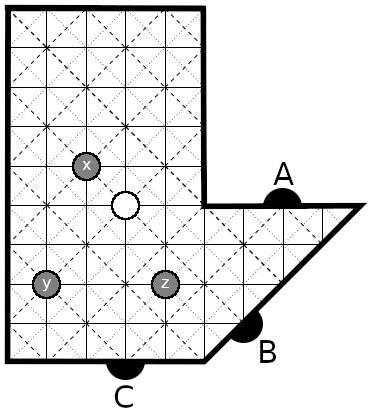
\includegraphics[width=\linewidth]{assets/Billiards_Puzzle_Tutorial.png}

The solution to this arena is zB-yC-xA. Solve each of the four other provided arenas, and enter each solution into ClueKeeper using this format.
